\documentclass{ecai}
\usepackage{times}
\usepackage{graphicx}
\usepackage{latexsym}
\usepackage{multirow}
\usepackage{amsmath}
\usepackage{xcolor}

%\ecaisubmission   % inserts page numbers. Use only for submission of paper.
                  % Do NOT use for camera-ready version of paper.

\begin{document}

\title{A General Neural Architecture for Carbohydrate and Bolus Recommendations in Type 1 Diabetes Management}

\author{Jeremy Beauchamp \and \ Razvan Bunescu \and Cindy Marling\institute{Ohio University, USA, email: \{jb199113,bunescu,marling\}@ohio.edu}}

\maketitle
\bibliographystyle{ecai}

\begin{abstract}
People with type 1 diabetes must constantly monitor their blood glucose levels and take actions to keep them from getting either too high or too low. Having a snack will raise blood glucose levels; however, the amount of carbohydrates that should be consumed to reach a target level depends on the recent history of blood glucose levels, meals, boluses, and the basal rate of insulin. Conversely, to lower the blood glucose level, one can administer a bolus of insulin; however, determining the right amount of insulin in the bolus can be cognitively demanding, as it depends on similar contextual factors. In this paper, we show that a generic neural architecture previously used for blood glucose prediction in a {\it what-if} scenario can be converted to make either carbohydrate or bolus recommendations. Initial experimental evaluations on the task of predicting carbohydrate amounts necessary to reach a target blood glucose level demonstrate the feasibility and potential of this general approach.
\end{abstract}

\section{Introduction and Motivation}

Type 1 diabetes is a disease in which the pancreas fails to produce insulin, which is required for blood sugar to be absorbed into cells. Without it, that blood sugar remains in the bloodstream, leading to high blood glucose levels (BGLs). In order to manage type 1 diabetes, insulin must be administered via an external source, such as injections or an insulin pump. People with type 1 diabetes also need to monitor their BGLs closely throughout the day by testing the blood acquired through fingersticks and/or by using a continuous glucose monitoring (CGM) system. If the BGL gets too high (hyperglycemia) or too low (hypoglycemia), the individual responds by eating, taking insulin, or taking some other action to help get their BGL back to within a healthy range. An issue with this, however, is that the person with diabetes must \emph{react} to their BGL, whereas, ideally, they would be able to \emph{proactively} control their BGL. There has been much work in the area of BGL prediction in the past (\cite{bunescu:icmla13} and \cite{plis:maiha14} for example) with the aim of enabling preemptive actions to manage BGLs before individuals experience the negative symptoms of hypoglycemia or hyperglycemia. However, individuals still need to figure out how much to eat, how much insulin to take, and what other actions they can take to prevent hypoglycemia or hyperglycemia.

The broad goal of the research presented in this paper is to essentially reverse the blood glucose prediction problem, and instead predict how many carbohydrates an individual should eat or how much insulin to administer with a bolus in order to get their BGL to the desired target. We have previously introduced in \cite{mirshekarian:embc19} an LSTM-based neural architecture that was trained such that it could answer {\it what-if} questions of the type “What will my BGL be in 60 minutes if I eat a snack with 30 carbs 10 minutes from now”. We show that by using the BGL target as a feature and the carbohydrates or insulin as labels, a similar architecture can be trained instead to predict the number of carbohydrates that need to be consumed or the amount of insulin that needs to be delivered during the prediction window in order to reach that BGL target.
% This essentially is the next step after the future BGL is predicted, the patient then needs to take action to either correct or maintain their BGL. This system can help patients make sure that they are taking the appropriate action to accomplish this. This is implemented using recurrent neural networks on data gathered from Type 1 Diabetes patients.

The work by Mougiakakou and Nikita \cite{stavroula:dtt} represents one of the first attempts to use neural networks for recommending insulin regimens and dosages. Bolus calculators were introduced as early as 2003 \cite{zisser:dtt08}, wherein a standard formula is used to calculate the amount of bolus insulin based on parameters such as carbohydrate intake, carbohydrate-to-insulin ratio, insulin on board, and target BGL. Walsh et al. \cite{walsh:jdst18} discuss major sources of errors and potential targets for improvement, such as utilizing the massive quantities of clinical data being collected by bolus advisors. As observed by Cappon et al.~in \cite{cappon:jdst18}, the standard formula approach ignores potentially useful preprandial conditions, such as the glucose rate of change. A feed-forward fully connected neural network was then proposed to exploit CGM information and some easily accessible patient parameters, with experimental evaluations on simulated data showing a small but statistically significant improvement in the blood glucose risk index. Simulated data is also used by Sun et al.~in \cite{sun:jbhi19}, where a basal-bolus advisor is trained using reinforcement learning in order to provide personalized suggestions to people with type 1 diabetes under multiple injections therapy.

The data-driven architecture proposed in this paper is generic in the sense that it can be trained to make recommendations about any variable that can impact BG levels, in particular carbohydrates and insulin. The task of making carbohydrate recommendations is potentially useful in scenarios where patients want to prevent hypoglycemia well in advance, or where a person is interested in achieving a relatively higher target BGL in preparation for an exercise event that is expected to lower it.

As a first step, in this paper we approach the problem of making carbohydrate recommendations.
% to demonstrate the feasibility of the proposed architecture.
The rest of this paper is organized in the following way: Section 2 provides a more detailed description of the problem. Section 3 describes the model as well as the baselines used to compare against. Section 4 describes the dataset that is used and some of the features of the data. Section 5 discusses some of the training techniques and methods used as well as the results of the experiments that motivated the use of these techniques. Section 6 contains the conclusion and some plans for future work.
 

\begin{figure*}[t]
    \centering
    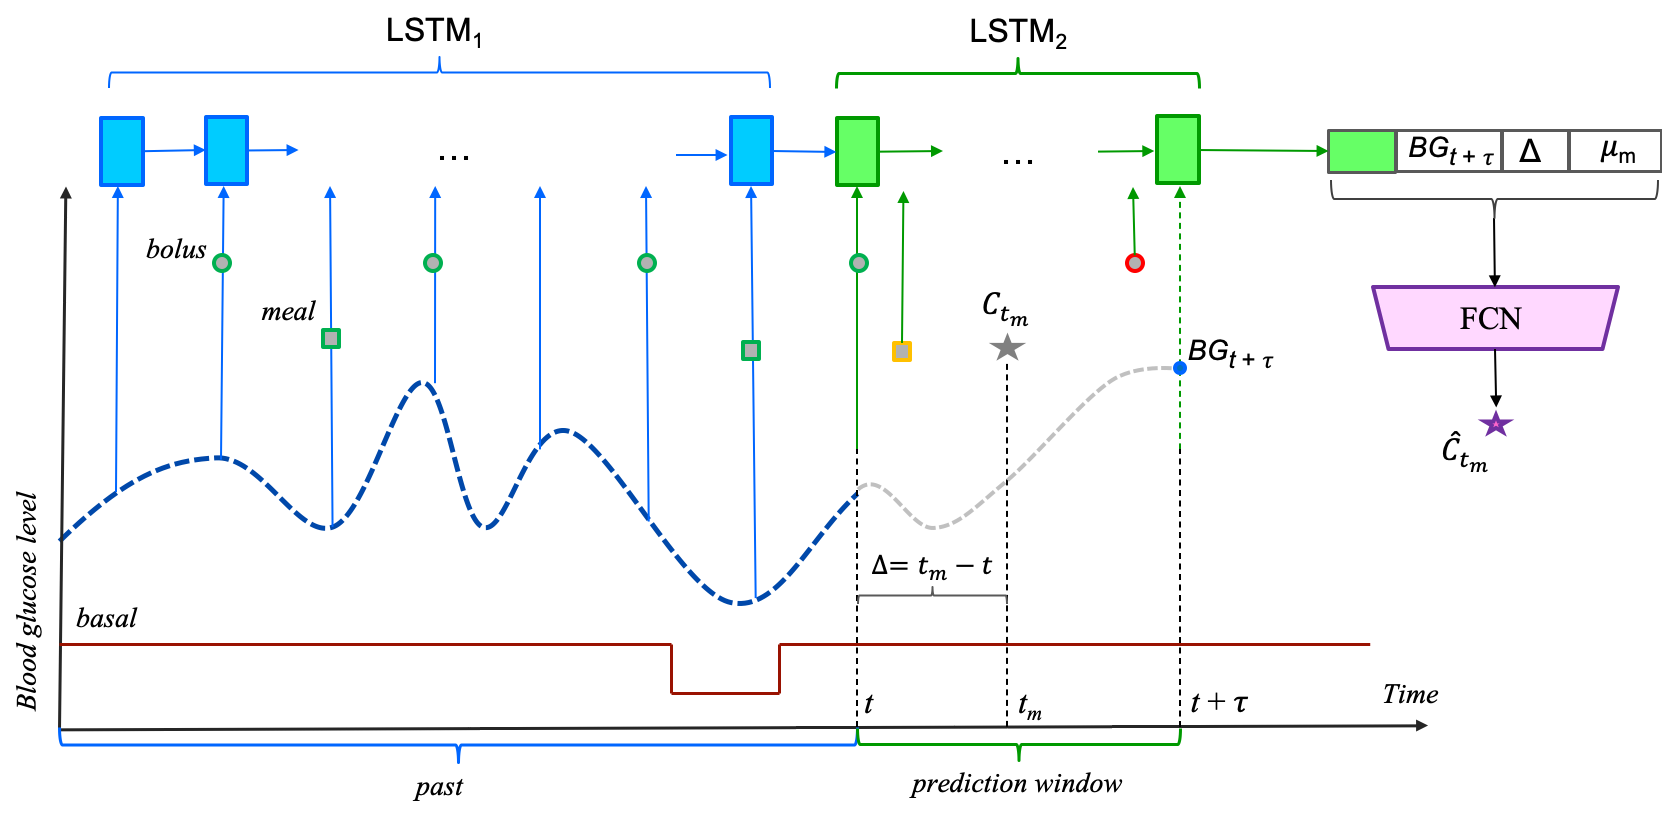
\includegraphics[width=0.9\textwidth]{kdh_paper_diagram}
    \caption{The general neural network architecture for carbohydrate recommendation. The dashed blue line in the graph represents a subject's BGL, while the solid brown line represents the basal rate of insulin. The gray star represents the meal at $t_{m}$. The other meals are represented by squares, and boluses are represented by circles. Meals and boluses with a green outline are allowed in all three example scenarios, while those with an orange outline are allowed in scenario $S_2$ and scenario $S_3$ examples, and those with a red outline are only allowed in scenario $S_3$ examples. The blue units in $\text{LSTM}_{1}$ receive input from different time steps in the past. The green units in $\text{LSTM}_{2}$ receive input from the prediction window. The purple trapezoid represents the 5 fully connected layers, whereas the output node at the end computes the carbohydrate prediction.}
    \label{fig:diagram}
\end{figure*}

\section{Three Carbohydrate Recommendation Scenarios}

We assume that blood glucose levels are measured at 5 minute intervals through a CGM system. We also assume that discrete deliveries of insulin (boluses) and continuous infusions of insulin (basal rates) are recorded. Subjects provide the timing of meals and estimates of the amount of carbohydrates associated with each meal. Given the data available up to the present time $t$, the problem can formally be defined as predicting the number of grams of carbohydrates (number of carbs) $C_{t_m}$ in a meal that is to be consumed at time $t_m \in [t, t + \tau)$ such that the person's BGL reaches a specified target value $BG_{t + \tau}$ at time $t + \tau$ in the future. Without loss of generality, in this paper we set the {\it prediction horizon} $\tau = 30$ and $60$ minutes. 
% However, the proposed approach is general and can be applied for other prediction horizons. 
We define three carbohydrate prediction scenarios, depending on whether events such as boluses or other meals happen inside the {\it prediction window} $[t, t + \tau)$:
% Along with these two given values, two sequences of data are used to make predictions. Consider $t_{0}$ to be $t_{m} + t_{t} - 30$, and $t_{0+30}$ to be $t_{m} + t_{t}$. This creates a 30 minute window around the meal. This first sequence, $\textbf{S}_{1}$, is a series of BGLs, the number of carbs eaten, and the amount of insulin taken each 5 minutes for 6 hours prior to $t_{0}$. The second sequence, $\textbf{S}_{2}$, is the series of the number of carbs eaten (excluding the meal at $t_{m}$), and the amount of insulin taken each 5 minutes from in the time frame $[t_{0}, t_{0+30})$.
\begin{enumerate}
	\item {\bf Scenario $\mathbf{S_1}$} assumes that there are no events in the prediction window $[t, t + \tau)$.  Training a model for this scenario can be difficult due to the scarcity of corresponding training examples, as meals are typically preceded by boluses. The example shown in Figure~\ref{fig:diagram} would be in this scenario if the orange and red outlined meals and boluses were not present.
	\item {\bf Scenario $\mathbf{S_2}$} subsumes scenario $S_{1}$ by allowing events before the meal, i.e. in the time window $[t, t_{m}]$. The example that is shown in Figure~\ref{fig:diagram} would be a scenario $S_{2}$ example if the bolus outlined in red were not present, and would correspond to answering the following {\it what-if} question: how many carbs should be consumed at time $t_m$ to achieve the target $BG_{t + \tau}$, if the meal were to be preceded by another meal and a bolus.
	\item {\bf Scenario $\mathbf{S_3}$} is the most general and allows events to happen during the entire prediction window $[t, t + \tau)$. The example in Figure~\ref{fig:diagram} is a scenario $S_{3}$ example but not a scenario $S_{1}$ or scenario $S_{2}$ example because of the presence of the orange and red outlined meal and bolus.
% 	These are the most plentiful class of examples, as each meal has exactly 6 corresponding examples, one for each possible value of $t_{t}$. This set is a superset of scenario 2 examples. 
\end{enumerate} 
We train and evaluate carbohydrate recommendation models for each scenario, using data acquired from 6 subjects with type 1 diabetes \cite{ohiot1dm:marling:kdh18}. Given the scarcity of training examples for scenario $S_{1}$, our starting hypothesis is that models that are trained on examples from scenario $S_{3}$ will implicitly learn physiological patterns that will improve performance for the fewer examples in scenario $S_{1}$.


%	\item The sequence of insulin, BGL readings, and meals 6 hours prior to $t_{0}$, $\textbf{S}_{1}$.
	
%	\item The sequence of insulin and meals (excluding the meal at $t_{m}$) between $t_{0}$ and $t_{0+30}$. This sequence is called $\textbf{S}_{2}$.
	
% Each example is labeled with the number of carbs in the meal at $t_{m}$, $y$.

\section{Baseline Models and Neural Architecture}

Given training data containing meals with their corresponding time-stamps and carbohydrates, we define the following baselines:
\begin{enumerate}
    \item {\bf Global average}: 
    The average number of carbs over all of the meals in the subject's training data, $\mu$, are computed and used as the estimate for all future meals, irrespective of context. This is a fairly simple baseline, as it predicts the same value for every example.
    
    %Compute the average number of carbs over all of the meals in the subject's training data, and use this average $\mu$ as the estimate for all future meals, irrespective of context. This is a fairly simple baseline, as it predicts the same value for every example.
    \item {\bf ToD average}: In this Time-of-Day (ToD) dependent baseline, an average number of carbs is computed for each of the following five time windows during a day:
	\begin{itemize}
		\item 12am-6am: $\mu_1$ = early breakfast/late snacks.
		\item 6am-10am: $\mu_2$ = breakfast.
		\item 10am-2pm: $\mu_3$ = lunch.
		\item 2pm-6pm: $\mu_4$ = dinner.
		\item 6pm-12am: $\mu_5$ = late dinner/post-dinner snacks.
	\end{itemize}
    The average for each ToD interval is calculated over all of the meals appearing in the corresponding time frame in the subject's training data. At test time, to predict the number of carbs for a meal to be consumed at time $t_m$, we first determine the ToD interval that contains $t_m$ and output the corresponding ToD average.
\end{enumerate}
Given sufficient historical data, the ToD baseline is expected to perform well for individuals who tend to eat very consistently and have regular diets. However, it is expected to perform poorly on individuals who have a lot of variation in their diets.

While simple to compute and use at test time, the two baselines are likely to give suboptimal performance, as their predictions ignore the history of BG values, insulin (boluses and basal rates), and meals, all of which could significantly modulate the effect a future meal might have on the BGL. To exploit this information, we propose the general neural network architecture shown in Figure~\ref{fig:diagram}. The first component in the architecture is a recurrent neural network (RNN) instantiated using Long Short-Term Memory (LSTM) cells \cite{hochreiter:nc97}, which is run over the previous 6 hours of data, up to the present time $t$. At each time step (5 minutes), this LSTM network takes as input the BGL, the carbohydrates, and the insulin dosages recorded at that time step. While sufficient for processing data corresponding to scenario $S_1$, this LSTM cannot be used to process events in the prediction window $[t, t + \tau)$ that may appear in scenarios $S_2$ and $S_3$, for which BGL values are not available. Therefore, in these scenarios, the final state computed by the first LSTM model (LSTM$_1$) at time $t$ is projected and used as the initial state for a second LSTM model (LSTM$_2$) that is run over the time steps between $(t, t+\tau)$. The final state computed either by LSTM$_1$ (for scenario $S_{1}$) or LSTM$_2$ (for scenarios $S_2$ and $S_3$) is then used as input to a fully connected network (FCN) whose output node computes $\hat{C}_{t_m}$, an estimate of the carbohydrates at time $t_m$. Besides the LSTM final state, the input to the FCN contains the following additional features: 
\begin{enumerate}
    \item The target BGL at $\tau$ minutes into the future, i.e. $BG_{t + \tau}$.
    \item The time interval $\Delta = t_m - t$ between the intended meal time and the present.
    \item The ToD average computed for Baseline 2 corresponding to the time the meal was eaten. 
\end{enumerate}
The entire architecture is trained to minimize the mean squared error between the actual carbohydrates $C_{t_m}$ recorded in the training data and the estimated value $\hat{C}_{t_m}$ computed by the output node of the FCN module. Each LSTM uses vectors of size 100 for the states and gates, whereas the FCN is built with 5 hidden layers, each consisting of 200 ReLU neurons, and one linear output node.

% Two slightly different models are trained to make these predictions. Both of them use recurrent networks and fully connected layers. Recurrent networks were chosen for their usefulness in processing time-series data. Long Short Term Memory (LSTM) networks were chosen specifically because the input sequences are quite long, and LSTMs are much better at handling long sequences than simple recurrent networks, as they can remember and forgot information as needed throughout the sequence.  

%The single LSTM model is used exclusively for scenario 1 examples. The double LSTM model is used for scenario 2 and scenario 3 examples,  but can also be used for scenario 1 examples. The models have much in common, so the more complex double LSTM model will be explained in full, and the single LSTM model will be explained in terms of the double LSTM model.

% The single LSTM model is very similar to the double LSTM model, with the only difference being that the single LSTM does not include $\text{LSTM}_{2}$. Instead, the output from the $\text{LSTM}_{1}$, $h'$ is concatenated with $\hat{bgl}$, $t_{t}$, and $\text{carb}_\text{avg}$ to create the vector \textbf{v}.



\section{Dataset}

The data used for the model was collected from 6 subjects with type 1 diabetes \cite{ohiot1dm:marling:kdh18}.  Information including the basal rate of insulin, boluses, meals, and BGL readings was collected over roughly 50 days, although the exact amount of time varies from subject to subject.  This time series data is split into three sets, as follows: the last 10 days of data for each subject are used as testing, the previous 10 days are used as validation, and the remainder of the data is used for training.

\subsection{From Meal Events to Examples }

Since the total number of available examples is directly related to the number of meals, it is useful to know how many meals each subject had. This is shown in Table \ref{tab:meals}, together with the average number of carbs per meal (Avg), and the corresponding standard deviation (StdDev).
\begin{table}
\begin{center}
\caption{Meal statistics, per subject and total.}
\label{tab:meals}
\begin{tabular}{|c|r|r|c|c|}
    \cline{3-4}
    \multicolumn{2}{c}{} & \multicolumn{2}{|c|}{Carbs Per Meal}\\
	\hline
	Subject & \multicolumn{1}{c|}{Meals} & \multicolumn{1}{c|}{Avg} & StdDev\\
	\hline
	559 & 179 & 36.0 & 16.0\\
    563 & 153 & 29.9 & 16.3\\
    570 & 169 & 105.3 & 42.0\\
	575 & 284 & 40.6 & 22.9\\
	588 & 257 & 30.8 & 16.6\\
	591 & 249 & 31.6 & 14.2\\
	\hline
	Total & 1291 & 43.5 & 33.1\\
	\hline

\end{tabular}
\end{center}
\end{table}
Most subjects have a similar average number of carbohydrates in their meals, with the exception of 570 who has a significantly larger number of carbs per meal on average, and more importantly, a much higher standard deviation than the other subjects. 
%This indicates that the models and baselines will likely perform worse on subject 570's examples than on any of the other subjects' examples. 

% There was one outlier meal that was removed from the data, specifically a meal in subject 588's validation data that contained 450 carbs. For reference, the next highest number of carbs found in a meal across the whole dataset was only 200 carbs. The outlier meal appeared to be a value that was incorrectly entered by the subject.

%\subsection{Example Counts}

A meal event occurring at time $t_m$ may give rise to multiple examples, depending on the position of $t_m$ in the interval $[t, t+\tau)$. When $\tau = 30$ minutes, an example is created for every possible position of $t_m$ within $[t, t+\tau)$. However, when $\tau = 60$ minutes, an example is created for every position of $t_m$ within $[t, t+30]$, to ensure that there are at least 30 minutes between the meal and the prediction horizon. Table \ref{tab:examples} below shows the resulting number of examples for $\tau = 30$ and 
$60$ minutes, in each of the three scenarios. Note that there are fewer examples in scenarios $S_1$ and $S_2$ when $\tau = 60$ vs. $30$ minutes, despite there being more scenario $S_3$ examples. This can be explained by the scenarios $S_1$ and $S_2$ criteria being even more difficult to meet when $\tau = 60$ minutes, i.e. there cannot be any event within $[t, t+60)$ for $S_1$, or any event within $[t_m, t+60)$ for $S_2$.

%A meal event occurring at time $t_m$ gives rise to multiple examples, depending on the position of $t_m$ in the interval $[t, t+\tau)$. Table \ref{tab:examples} below shows the number of examples corresponding to each scenario.

\begin{table}
\begin{center}
\caption{Example counts by scenario, for 30 and 60 minutes.}
\label{tab:examples}
\begin{tabular}{|l|r|r|r|r|r|r|}
	\cline{2-7}
	\multicolumn{1}{c}{} & \multicolumn{2}{|c}{Scenario $S_1$} & \multicolumn{2}{|c}{Scenario $S_2$} & \multicolumn{2}{|c|}{Scenario $S_3$}\\
	\hline
	Dataset & \multicolumn{1}{c|}{30} & \multicolumn{1}{c|}{60} & \multicolumn{1}{c|}{30} & \multicolumn{1}{c|}{60} & \multicolumn{1}{c|}{30} & \multicolumn{1}{c|}{60}\\
	\hline
	Training & 2396 & 1923 & 3889 & 3491 & 5096 & 5931\\
	Validation & 629 & 510 & 1061 & 981 & 1388 & 1626\\
	Testing & 469 & 339 & 950 & 851 & 1236 & 1435\\
	\hline
	Total & 3494 & 2772 & 5900 & 5323 & 7720 & 8992\\
	\hline
\end{tabular}
\end{center}
\end{table}

% Only 20\% of the examples in the dataset meet the criteria to be considered scenario 1 examples. With such a low number of examples, it is difficult to train a model to perform such a complex task.  Since scenario 2 and scenario 3 examples have all of the features that are required for the models to train and make predictions, training on these examples could help a model to perform better on scenario 1 examples.

\section{Experimental Evaluation}

The Adam \cite{kingma:adam} variant of gradient descent is used for training, with the learning rate and mini-batch size being tuned on the validation data. In an effort to avoid overfitting, early stopping with a patience of 5 epochs and dropout with a rate of 10\% are used for both models. Interestingly, dropout was found to help the model if it was only applied to the LSTM networks of the model at each time step and not the fully connected network.

Since the overall number of examples available in the dataset is low, the performance was improved by first pretraining a generic model on the combined data from all 6 subjects. Then, for each subject, a new model is initialized with the weights of the generic model, and then fine-tuned on the subject's training data. For each subject, five models were trained with different seedings of the random number generators. We also experimented with fine-tuning models on the union of the training and validation data instead of just the training data.  When this combined data is used, the average carb values used in the baselines are recalculated over the union of the training and validation data for each subject.

\subsection{Results}

The metrics used to evaluate the performance of the models are the root mean squared error (RMSE) and the mean absolute error (MAE), which is less sensitive to large errors. 
At the end of the training process, there are five fine-tuned models for each subject. The {\it average} RMSE and MAE of the five models are reported, as well as the RMSE and MAE of the {\it best} model. The model that is considered the "best" is the one that had the lowest MAE on the validation data. The results of the five models for each subject are also averaged across all subjects to obtain one overall RMSE and one overall MAE value for the \textit{average model} and the \textit{best model} scores. The baselines are treated much the same, as their RMSE and MAE values are averaged across all subjects to give an RMSE and an MAE score for each baseline. %{\color{blue} The prediction horizon, $\tau$, is 30 minutes unless it is specifically stated otherwise.}  % This makes it easy to compare in a general sense how the models perform relative to the baselines.

Table \ref{tab:pretraining} compares the validation results achieved in scenario $S_3$ by models with and without pretraining for $\tau = 30$ minutes. This experiment clearly shows the benefit of pretraining the models: both the RMSE and MAE are noticeably lower for the pretrained models. As a result, pretraining is always used as part of the training process for both values of $\tau$.
\begin{table}
\begin{center}
\caption{Results with and without pretraining, $\tau = 30$.}
\label{tab:pretraining}
\begin{tabular}{|c|c|c|c|}

	\hline
	Setting & RMSE & MAE\\
	\hline
	Without Pretraining & 22.2 & 15.5\\	   				  
	With Pretraining & \textbf{20.7} & \textbf{14.5}\\
	\hline

\end{tabular}
\end{center}
\end{table}

Table \ref{tab:combined} compares models that were fine-tuned on training and validation data with models fine-tuned solely on the training data, in scenario $S_3$. The results show that the extra examples provided by the validation data proved helpful in improving performance. It is interesting to note that using the combined training-validation data only slightly helped the baselines, but helped the LSTM-based models by a noticeable margin.
\begin{table}
\begin{center}
\caption{Fine-tuning on Training vs. Training $\cup$ Validation, $\tau = 30$.}
\label{tab:combined}
\begin{tabular}{|l|c|c|c|}

	\hline
	Fine-tuning & Baselines \& Models & RMSE & MAE\\
	\hline
	\multirow{4}{*}{Training} & Global Average & 23.3 & 19.2\\
							 & ToD Average & 22.5 & 17.8\\
							 \cline{2-4}
							 & Average Model & 21.3 & 16.0\\
							 & Best Model & \textbf{20.7} & \textbf{15.3}\\
	\hline
	& Global Average & 23.1 & 19.0\\
						  Training $\cup$ & ToD Average & 22.2 & 17.7\\
						  \cline{2-4}
						  \ \ \ \ Validation & Average Model & 20.1 & 15.0\\
						  & Best Model & \textbf{19.2} & \textbf{14.2}\\
	\hline			   

\end{tabular}
\end{center}
\end{table}


%Table \ref{tab:all_results} shows the performance on test data in each of the three scenarios. Subject 570 was excluded from this experiment, due to the scarcity of examples in scenario 1, in particular just 1 validation example and 5 test examples. 

Table~\ref{tab:all_results} compares the Baselines (Global and ToD averages) with the trained Models (Best and Average) in terms of their RMSE and MAE in the three scenarios.
\begin{table}
\caption{Results for scenarios $S_{1}$, $S_{2}$, and $S_{3}$, for $\tau = 30$ and 60 minutes.}
\begin{center}
\label{tab:all_results}
\begin{tabular}{|c|c|c|c|c|c|}

   	\cline{3-6}
	\multicolumn{2}{c}{} & \multicolumn{2}{|c|}{RMSE} & \multicolumn{2}{c|}{MAE}\\
	\cline{2-6}
	\multicolumn{1}{c|}{} & Baselines \& Models & 30 & 60 & 30 & 60\\
	\hline
	\multirow{4}{*}{$S_{1}$} & Global Average & 19.7 & 18.4 & 15.7 & 15.0\\
					   & ToD Average & \textbf{18.9} & \textbf{17.6} & 14.8 & 14.4\\
					   \cline{2-6}
					   & Average Model & 19.3 & 19.5 & 14.1 & \textbf{13.9}\\
					   & Best Model & 19.0 & 19.8 & \textbf{13.9} & \textbf{13.9}\\
	\hline
	\multirow{4}{*}{$S_{2}$} & Global Average & 18.4 & 17.1 & 14.5 & 13.8\\
					   & ToD Average & 17.4 & 15.9 & 13.1 & 12.2\\
					   \cline{2-6}
					   & Average Model & 16.2 & \textbf{15.3} & 11.9 & 11.4\\
					   & Best Model & \textbf{15.8} & 15.4 & \textbf{11.6} & \textbf{10.9}\\
	\hline
	\multirow{4}{*}{$S_{3}$} & Global Average & 18.5 & 18.6 & 14.6 & 14.7\\
					   & ToD Average & 17.5 & 17.6 & 13.2 & 13.3\\
					   \cline{2-6}
					   & Average Model & 15.7 & 15.6 & 11.5 & 11.3\\
					   & Best Model & \textbf{15.6} & \textbf{14.8} & \textbf{11.4} & \textbf{10.6}\\
	\hline
	

\end{tabular}
\end{center}
\end{table}
%The scenario 3 models had the best performance of all in both the average model score and the best model score. However, scenario 2 had quite similar results in all metrics for both the models and the baselines. The models for these scenarios outperformed both baselines in all aspects. However, the scenario 1 results are quite different from the other two scenarios. Both baselines performed worse than they did for scenario 2 and scenario 3 examples. This decline in performance is even more apparent when observing the model's performance, which is substantially worse than for the other scenarios. Neither the average model nor best model were able to beat the time-dependent baseline in terms of RMSE.

Overall, the LSTM-based models (Average or Best) had the best RMSE and MAE performance across all three scenarios, with the exception of the RMSE scores for scenario $S_1$. Compared to the other two scenarios, the LSTM models and the baselines have a lower performance in $S_1$. The decline in performance is even more apparent for the LSTM models, which cannot beat the time-dependent baseline in terms of RMSE for both the 30 minute and 60 minute prediction horizons. This can be explained by the limited number of examples for scenario $S_1$: since there are so few testing examples in this scenario per subject, one bad prediction can hurt the results significantly, more so for the RMSE than the MAE. Furthermore, the trained models tend to make very similar predictions for all examples stemming from a specific meal, meaning that if the model made a bad prediction for one test example, it likely made a series of similarly bad predictions.

To alleviate the scarcity of training examples in scenario $S_1$, models trained on $S_3$ examples, which are the most plentiful and subsume $S_1$, were evaluated separately on test examples from $S_1$. This gives an indication on whether any transfer learning is taking place. Table \ref{tab:case3_case1} shows the results of this transfer learning experiment, indicating that training on the additional examples from scenario $S_3$ helps improve performance on scenario $S_1$ to the level that now the LSTM-based models outperform both baselines.% This is an important result, indicates that with more examples, the model should be expected to perform better. 

%Finally, Table \ref{tab:case3_case1} shows the results of the transfer learning experiment, where models trained on scenario 3 examples are also evaluated only on scenario 1 examples. The results show that training on the additional examples from scenario 3 helps improve performance on scenario 1 to the level that now the proposed model outperforms both baselines.% This is an important result, indicates that with more examples, the model should be expected to perform better. 

\begin{table}
\caption{Comparative performance on scenario $S_1$ test examples: Baselines vs. LSTM-based models trained on $S_{1}$ and $S_{3}$ examples.}
\begin{center}
\label{tab:case3_case1}
\begin{tabular}{|c|c|c|c|c|c|}
	
    \cline{3-6}
	\multicolumn{2}{c}{} & \multicolumn{2}{|c|}{RMSE on $S_1$} & \multicolumn{2}{c|}{MAE on $S_1$}\\
	\cline{2-6}
	\multicolumn{1}{c|}{} & Baselines \& Models & 30 & 60 & 30 & 60\\
	\cline{2-6}
	\multicolumn{1}{c|}{} & Global Average & 19.7 & 18.4 & 15.7 & 15.0\\
    \multicolumn{1}{c|}{} & ToD Average & 18.9 & 17.6 & 14.8 & 14.4\\
	\hline 
	\multirow{2}{*}{Training on $S_{1}$} & Average Model & 19.3 & 19.5 & 14.1 & 13.9\\
	& Best Model & 19.0 & 19.8 & 13.9 & 13.9\\
	\hline
	\multirow{2}{*}{Training on $S_{3}$} & Average Model & \textbf{18.2} & 17.6 & \textbf{13.6} & 13.3\\
    & Best Model & 18.3 & \textbf{16.7} & 13.8 & \textbf{13.0}\\
	\hline
	

\end{tabular}
\end{center}
\end{table}


% For each table, the best RMSE and MAE for each experimental setting are bolded, and the best RMSE and MAE overall are bolded and italicized.

%The usefulness of pretraining was measured by evaluating five trained models with pretraining, and five trained models without pretraining for each subject. The hyper-parameter tuning phase was skipped for this experiment and the learning rate and mini-batch size were set to 0.001 and 32 respectively for all models. The results in Table \ref{tab:pretraining} are the average model scores on scenario 3 examples in the validation data with and without pretraining.


%Another technique that was tested was the use of the union of the training and validation data to fine-tune the models. To ensure that the baselines reflect this change, the averages used for making the baseline predictions are re-calculated across the union of the training and validation data. Table \ref{tab:combined} shows the RMSE and MAE on the testing data with and without using the combined training-validation data for fine-tuning the models. The models were evaluated on scenario 3 examples from the testing data.

%The next experiment shows the performance difference between models trained and evaluated on scenario 1, scenario 2, and scenario 3 examples. For this particular experiment, subject 570's models are not included for any scenario. This is because subject 570 has only 43 scenario 1 examples, and of the 43 there is only 1 validation example and 5 testing examples. This is not enough to get a meaningful measure of how the model is performing. The results in Table \ref{tab:comparison} were produced from the models being evaluated on testing data.




%\section{Related Work}
%The goal of carbohydrate prediction was inspired by the "what-if" scenario described in \cite{mirshekarian:embc19}, where a model would attempt to predict an individual's BGL an hour into the future if the individual ate a given number of carbs a given number of minutes into the future. The problem discussed in this paper essentially reverses this scenario by using the future BGL as a feature to predict the number of carbs in the meal.

%There has been research into meal recommendation systems for people with diabetes in the past. The approach described in this paper is not a recommendation system in the truest sense as it is treated as a regression problem, even though in practice the system would be giving recommendations. However, they are still closely related when considering the end goal of the systems. For example, the research  presented in \cite{norouzi:article} describes a meal recommendation system in which meals are recommended based on a person's preferences and conditions. This paper differs in the general approach to the problem, as it used a knowledge-based approach rather than a machine learning one, and takes into account information about the person's condition rather than their recent biological history.

%There also has been research into a similar problem using a similar approach, recommending an insulin regime to people with diabetes using neural networks \cite{stavroula:dtt}. This is a very similar problem as both are methods of changing the BGL of a person with diabetes. Carbohydrates can be used to raise the BGL while insulin can lower it. However, the problem was treated as a softmax problem, predicting which regime out of six was the best fit for an individual. Their approach also took the patient's recent BGLs and insulin intake into consideration when making predictions.

\section{Conclusion and Future Work}

We introduced a generic neural architecture, composed of two chained LSTMs and a fully connected network, with the purpose of training data-driven models for making recommendations with respect to any type of quantitative events that may impact BG levels, in particular carbohydrate amounts and bolus insulin dosages. Experimental evaluations on the task of carbohydrate recommendations within a 30 or 60 minute prediction window demonstrate the feasibility and potential of the proposed architecture, as well as its ability to benefit from pre-training and transfer learning. Future plans include evaluating carbohydrate recommendations within larger prediction windows, as well as training the architecture for bolus recommendations.

\ack This work was supported by grant 1R21EB022356 from the National Institutes of Health (NIH).  Conversations with Josep Vehi helped shape the research directions presented herein.  The contributions of physician collaborators Frank Schwartz, MD, and Amber Healy, DO, are gratefully acknowledged.  We would also like to thank the anonymous people with type 1 diabetes who provided their blood glucose, insulin, and meal data.

\bibliography{kdh20}
\end{document}
